\chapter{Implementation}
\label{ch:implementation}


\section{Development approach}
\label{sect:dev_approach}

The levels on which testing can occur as defined in \cite{Myers2004AST} are Unit testing (Module testing), Integration testing as well as Functional (overarching) testing...

	\subsection{Agile}
	\label{ssect:agile}
	
	\subsection{scrum}
	\label{ssect:scrum}
	
	\subsection{What I did...}
	\label{ssect:change_me}
	
	
	
\section{Web Development approach}
\label{sect:webdev_approach}


\begin{figure}[ht]
	\label{fig_webdev_approach}
	% \centering
	\hspace*{-0.5cm}
	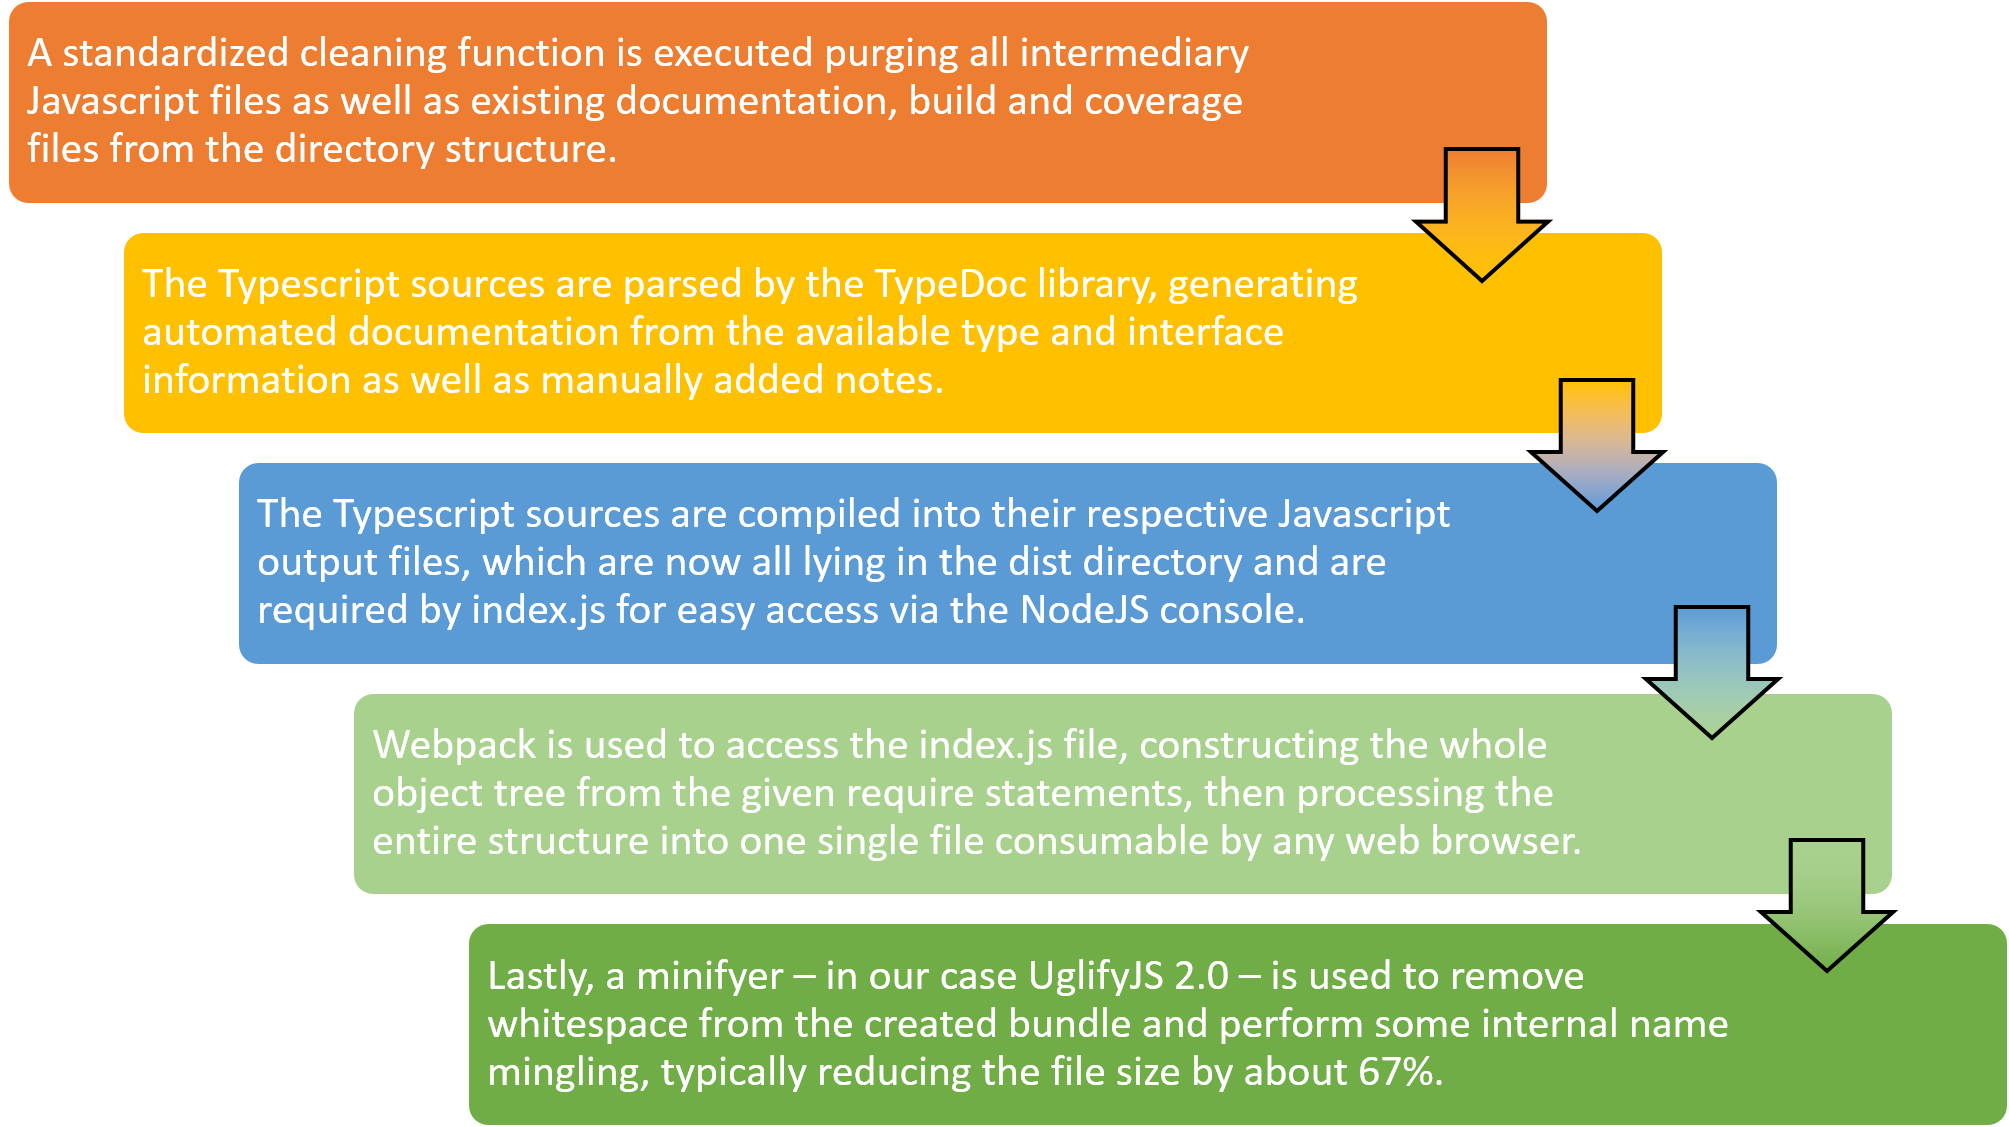
\includegraphics[width=1.1\textwidth]{figures/bundle_process}
	\caption{The GraphiniusJS Bundling process}
\end{figure}



\section{Testing approach}
\label{sect:testing_approach}

	BDD...
	
	\subsection{Unit tests}
	\label{ssect:unittests}
	
	\subsection{Functional tests}
	\label{ssect:func_tests}
	
	\subsection{GUI / Integration tests}
	\label{ssect:int_tests}


\section{Data Models}
\label{sect:data_models}

	\subsection{Users}
	\label{ssect:users}
	
	\subsection{Experiments}
	\label{ssect:experiments}
	
	\subsection{Algorithms}
	\label{ssect:algorithms}

	\subsection{Profile / Settings}
	\label{ssect:settings}


\section{Implemented Algorithms}
\label{sect:implemented_algos}

	\subsection{Core Search - BFS / DFS}
	\label{ssect:bfs_dfs}
	
	\subsection{Topological Sorting / SCC}
	\label{ssect:toposort_scc}
	
	\subsection{Degree Distribution}
	\label{ssect:deg_dist}
	
	\subsection{Centralities}
	\label{ssect:centralities}
	
	\subsection{Shortest paths}
	\label{ssect:shortest_paths}
	
	\subsection{Clustering}
	\label{ssect:clustering}
